\section{Verification}
\label{sec:verification}

\begin{figure*}[t]
\scriptsize{
\medskip
%%%%%%%%%%%%%%%%%%%%
$
\inferrule
{
}
{\Refines;\SkipProcs;\AvailableActions \vdash \skipstmt \leadsto \skipstmt}
\;(\textsc{Skip})
$
\medskip
%%%%%%%%%%%%%%%%%%%%
$
\inferrule
{
}
{\Refines;\SkipProcs;\AvailableActions \vdash \yield{e,\lins} \leadsto \yield{e',\lins'}}
\;(\textsc{Yield})
$
\medskip
%%%%%%%%%%%%%%%%%%%%
$
\inferrule
{
A \in \AvailableActions
}
{\Refines;\SkipProcs;\AvailableActions \vdash \call{A} \leadsto \call{A}}
\;(\textsc{Atomic})
$
\medskip
%%%%%%%%%%%%%%%%%%%%
$
\inferrule
{
\Refines;\SkipProcs;\AvailableActions \vdash s \leadsto s'
}
{
\Refines;\SkipProcs;\AvailableActions \vdash \ablock{e,\lins}{s} \leadsto s'
}
\;(\textsc{Ablock1})
$
\medskip
%%%%%%%%%%%%%%%%%%%%
$
\inferrule
{
\Refines;\SkipProcs;\AvailableActions \vdash s \leadsto s'
}
{
\Refines;\SkipProcs;\AvailableActions \vdash s \leadsto \ablock{e,\lins}{s'}
}
\;(\textsc{Ablock2})
$
\medskip
%%%%%%%%%%%%%%%%%%%%
$
\inferrule
{
P \in \dom(\Refines)
}
{
\Refines;\SkipProcs;\AvailableActions \vdash \call{P} \leadsto \call{\Refines(P)}
}
\;(\textsc{Proc1})
$
\medskip
%%%%%%%%%%%%%%%%%%%%
$
\inferrule
{
P \in \SkipProcs
}
{
\Refines;\SkipProcs;\AvailableActions \vdash \call{P} \leadsto \skipstmt
}
\;(\textsc{Proc2})
$
\medskip
%%%%%%%%%%%%%%%%%%%%
$
\inferrule
{
P \not\in \dom(\Refines) \cup \SkipProcs
}
{
\Refines;\SkipProcs;\AvailableActions \vdash \call{P} \leadsto \call{P}
}
\;(\textsc{Proc3})
$
\medskip
%%%%%%%%%%%%%%%%%%%%
$
\inferrule
{
P \in \SkipProcs
}
{
\Refines;\SkipProcs;\AvailableActions \vdash \async{P} \leadsto \skipstmt
}
\;(\textsc{Async1})
$
\medskip
%%%%%%%%%%%%%%%%%%%%
$
\inferrule
{
P \not\in \dom(\Refines) \cup \SkipProcs
}
{
\Refines;\SkipProcs;\AvailableActions \vdash \async{P} \leadsto \async{P}
}
\;(\textsc{Async2})
$\\
\medskip
%%%%%%%%%%%%%%%%%%%%
$
\inferrule
{
\Refines;\SkipProcs;\AvailableActions \vdash s_1 \leadsto s_1' \\
\Refines;\SkipProcs;\AvailableActions \vdash s_2 \leadsto s_2'
}
{
\Refines;\SkipProcs;\AvailableActions \vdash \ite{\locExpr}{s_1}{s_2} \leadsto \ite{\locExpr}{s_1'}{s_2'}
}
\;(\textsc{Ite})
$
\medskip
%%%%%%%%%%%%%%%%%%%%
$
\inferrule
{
\Refines;\SkipProcs;\AvailableActions \vdash s \leadsto s'
}
{
\Refines;\SkipProcs;\AvailableActions \vdash \while{e,\alpha}{\locExpr}{s} \leadsto \while{e',\alpha'}{\locExpr}{s'}
}
\;(\textsc{While})
$
\medskip
%%%%%%%%%%%%%%%%%%%%
$
\inferrule
{
\Refines;\SkipProcs;\AvailableActions;b \vdash \StmtStack \leadsto \StmtStack' \\
\Refines;\SkipProcs;\AvailableActions \vdash \stmt \leadsto \stmt'
}
{
\Refines;\SkipProcs;\AvailableActions;b \vdash \StmtStack;\stmt \leadsto \StmtStack';\stmt'
}
\;(\textsc{Seq})
$
\medskip
%%%%%%%%%%%%%%%%%%%%
$
\inferrule
{
P \in \dom(\Refines)
}
{
\Refines;\SkipProcs;\AvailableActions;\false \vdash (P,\varsL,\StmtStack) \leadsto \yield{e,\lins}; \call{\Refines(P)}; \yield{e',\lins'}
}
\;(\textsc{Stack1})
$
\medskip
%%%%%%%%%%%%%%%%%%%%
$
\inferrule
{
P \in \dom(\Refines) \cup \SkipProcs
}
{
\Refines;\SkipProcs;\AvailableActions;\true \vdash (P,\varsL,\StmtStack) \leadsto \yield{e',\lins'}
}
\;(\textsc{Stack2})
$
\medskip
%%%%%%%%%%%%%%%%%%%%
$
\inferrule
{
P \not \in \dom(\Refines) \cup \SkipProcs \\
\Refines;\SkipProcs;\AvailableActions;b \vdash \StmtStack \leadsto \StmtStack'
}
{
\Refines;\SkipProcs;\AvailableActions;b \vdash (P,\varsL,\StmtStack) \leadsto (P,\varsL,\StmtStack')
}
\;(\textsc{Stack3})
$
\medskip
%%%%%%%%%%%%%%%%%%%%
$
\inferrule
{
\Refines;\SkipProcs;\AvailableActions \vdash \stmt \leadsto \stmt'
}
{
\Refines;\SkipProcs;\AvailableActions \vdash (\phi,\mods,\psi,\stmt) \leadsto (\phi',\mods',\psi',\stmt')
}
\;(\textsc{Procedure})
$
\medskip
%%%%%%%%%%%%%%%%%%%%
$
\inferrule
{
\Refines;\SkipProcs;\AvailableActions;b \vdash (P, \varsL, \StmtStack) \leadsto \StmtStack'
}
{
\Refines;\SkipProcs;\AvailableActions;b \vdash (\varsTL, (P, \varsL, \StmtStack)) \leadsto (\varsTL, \StmtStack')
}
\;(\textsc{Thread})
$
\medskip\\
%%%%%%%%%%%%%%%%%%%%
$
\inferrule
{
\dom(\Refines) \cap \SkipProcs = \{ \} \\
\cod(\Refines) \subseteq \AvailableActions \\
\forall A \in \AvailableActions.\ \actions(A) = \actions'(A) \\\\
\forall (\rho,\alpha,m) \in \cod(\Refines \circ \actions).\ (\accessVars(\rho) \cap \Local = \emptyset) \wedge (\alpha = ((\elim{\Local}.\ \alpha) \wedge \Same(\Local))) \\\\
\forall 1 \le i \le n.\ \Refines;\SkipProcs;\AvailableActions;b_i \vdash T_i \leadsto T_i' \\
\forall P \not\in \dom(\Refines) \cup \SkipProcs.\ \Refines;\SkipProcs;\AvailableActions \vdash \procs(P) \leadsto \procs'(P)
}
{
\Refines;\SkipProcs;\AvailableActions;b_1;\ldots;b_n \vdash (\procs, \actions, \ProcLins, \varsG, T_1 \ldots T_n) \leadsto (\procs', \actions', \ProcLins', \varsG, T_1' \ldots T_n')
}
\;(\textsc{Program})
$
\medskip
%%%%%%%%%%%%%%%%%%%%
}
\caption{Program transformation}
\label{fig:program-transformation}
\end{figure*}

Suppose a program $\Prog'$ has been proved to be safe.
However, it is implemented using atomic actions that are too coarse to be directly implementable.  
To carry over the safety of $\Prog'$ to a realizable implementation $\Prog$, 
these coarse atomic actions must be refined down to lower-level actions.
During this refinement, an invocation $\call{A}$ of a high-level atomic action $A$ is transformed into an 
invocation $\call{P}$ of a procedure that is implemented using low-level actions.
The main contribution of this paper is a verification method that allows us to safely refine
program $\Prog'$ to another program $\Prog$ (or abstract $\Prog$ to $\Prog'$) so that 
safety properties proved on $\Prog'$ continue to hold on $\Prog$ as well.

We formalize the program transformation connecting $\Prog$ to $Prog'$ as a judgment
$\Refines;\SkipProcs;\AvailableActions \vdash \Prog \leadsto \Prog'$ (see rules in Figure~\ref{fig:program-transformation}).
In this judgment,
$\Refines \in \ProcName \pf \ActionName$ is a partial function from procedure names to action names
and $\AvailableActions \in 2^{\ActionName}$ is a set of action names.
This judgment expresses the intention that $\Prog$ is abstracted by replacing
occurrences of $\call{P}$ with $\call{\Refines(P)}$ for all $P \in \dom(\Refines)$ such that 
the resulting program $\Prog'$ uses only actions in $\AvailableActions$.
Consequently, the procedures in $\dom(\Refines)$ are not used in $\Prog'$.

Rule \textsc{Program} checks that $\cod(\Refines) \subseteq \AvailableActions$,
which ensures that $\Prog'$ only uses actions in $\AvailableActions$.
It also checks that every action in $\cod(\Refines)$ has a gate 
that is independent of procedure-local variables and a transition relation that leaves 
procedure-local variables unchanged.  
This check is meaningful because the action $\Refines(P)$ is written from the 
perspective of the caller of $P$.
Since the procedure-local variables of the caller of $P$ are distinct from those of $P$,
these variables are quantified out from the transition relation of $\Refines(P)$ when 
the body of $P$ is being checked (see Section~\ref{sec:refinement}).
Finally, this rule constrains actions in $\AvailableActions$ to be identical in $\Prog$ and $\Prog'$ and then rewrites all threads
and all procedures that are still used in $\Prog'$.

If $P \in \dom(\Refines)$, rule \textsc{Proc1} rewrites $\call{P}$ to $\call{\Refines(P)}$;
otherwise, rule \textsc{Proc2} leaves $\call{P}$ unchanged.
Rule \textsc{Async} leaves the call unchanged but checks that $P \not \in \dom(\Refines)$.
Rule \textsc{Ablock2} breaks up atomic blocks that contain calls
to atomic actions that are being refined to procedures.
Rule \textsc{Ablock1} allows smaller atomic blocks to be created in the refined program.
Rule \textsc{Atomic} checks that $A \in \AvailableActions$ before leaving $\call{A}$ unchanged;
this rule ensures that the abstract program only uses actions in $\AvailableActions$.

The program transformation $\Prog \leadsto \Prog'$ is clearly not sound by itself.
To justify the transformation, a collection of auxiliary judgments need to be proved.
We now present an overview of these judgments.
The judgment $\vdash \Prog$, described in Section~\ref{sec:linearity}, 
checks that $\Prog$ uses linear variables appropriately and that the statement
inside any atomic block does not contain any yield.
The former is important because appropriate use of linear variables gives our verifier access to free disjointness
assumptions that are important for commutativity reasoning (Section~\ref{sec:yield-elimination})
and precise non-interference (Section~\ref{sec:refinement}).
The latter is important because non-interference between threads is checked pairwise by verifying that each yield predicate
in one thread is preserved by each atomic block in a different thread.

Next, we have two judgments $\CommutativitySafe(\Prog)$ and $\Refines \jy \Prog$, collectively 
referred to as {\em yield elimination\/} and described in Section~\ref{sec:yield-elimination}.
These judgments allow us to reduce the complexity of annotations and invariants 
required for proving the correctness of the concrete program $\Prog$
by justifying the absence of (implicit) yields between some of the 
invocations of atomic actions.
We use commutativity reasoning on definitions of atomic actions and their declared mover types~\cite{FlanaganFLQ08,ElmasQT09}
to perform yield elimination soundly.

Finally, we have two judgments, $\InterferenceSafe(\Prog)$ and $\Refines;\SkipProcs \jr \Prog$,
described in Section~\ref{sec:refinement},
that together establish that all program annotations are consistent and that 
each occurrence of $\call{P}$ in $\Prog$ behaves like $\call{\Refines(P)}$ 
for all $P \in \dom(\Refines)$.
The rules for these judgments generalize the method of Owicki and Gries~\cite{OwickiG76} for reasoning about concurrent programs.
The judgment $\InterferenceSafe(\Prog)$ checks that each thread preserves the
yield predicate of every other thread.
The judgment $\Refines;\SkipProcs \jr \Prog$ checks sequential correctness of each computation
and that the code of procedure $P$ behaves like the atomic action $\Refines(P)$ for all $P\in\dom(\Refines)$.

\begin{theorem}
\label{thm:correctness}
Let $\Prog,\Prog' \in \CProgram$ be such that $\vdash \Prog$ and $\vdash \Prog'$.
Let $\Refines \in \ProcName \pf \ActionName$, $\SkipProcs \in 2^{\ProcName}$, $\AvailableActions \in 2^{\ActionName}$,
and $\bs{b} \in \overrightarrow{\mathit{Boolean}}$ be such that the following conditions hold:
\begin{enumerate}
\item
$\Refines;\SkipProcs;\AvailableActions;\bs{b} \vdash \Prog \leadsto \Prog'$.
\item
$\jy \Prog$ and $\CommutativitySafe(\Prog)$.
\item
$\Refines;\SkipProcs;\bs{b} \jr \Prog$ and $\InterferenceSafe(\Prog)$.
\end{enumerate}
If $\Cooperative^*(\Prog)$ and $\Safe^*(\Prog')$, then $\Safe^*(\Prog)$.
\end{theorem}

Our soundness theorem, stated above, concludes the safety of $\Prog$ from the safety of $\Prog'$ 
and the responsiveness of $\Prog$.
In general, the correctness proof of a large program is obtained by chaining together
multiple instances of this theorem connecting a sequence of programs.  
The code of adjacent programs in this chain are constrained by the $\leadsto$ relation but the annotations are left 
unconstrained to allow as much flexibility in verification as possible.

\subsection{Using linear variables}
\label{sec:linearity}

\begin{figure*}[t]
\scriptsize{
\medskip
%%%%%%%%%%%%%%%%%%%%
$
\inferrule
{
}
{
\lins;\ABlockAny \vdash \skipstmt : \lins
}
\;(\textsc{Skip})
$
\medskip
%%%%%%%%%%%%%%%%%%%%
$
\inferrule
{
\lins_y \subseteq \lins
}
{
\lins;\ABlockOutside \vdash \yield{e,\lins_y} : \lins
}
\;(\textsc{Yield})
$
\medskip
%%%%%%%%%%%%%%%%%%%%
$
\inferrule
{
\ProcLins(A) = (\lins,\lins')
}
{
\lins;\ABlockInside \vdash \call{A} : \lins'
}
\;(\textsc{Atomic})
$
\medskip
%%%%%%%%%%%%%%%%%%%%
$
\inferrule
{
\ProcLins(P) = (\lins,\lins') \\
}
{
\lins;\ABlockOutside \vdash \call{P} : \lins'
}
\;(\textsc{Proc})
$
\medskip
%%%%%%%%%%%%%%%%%%%%
$
\inferrule
{
\lins_G \subseteq \Global \\
\lins \cup \lins_P \cup \lins_P' \subseteq \ThreadLocal \\
\ProcLins(P) = ((\lins_G,\lins_P),(\lins_G,\lins_P')) \\
}
{
\lins_G,\lins,\lins_P;\ABlockOutside \vdash \async{P} : \lins_G,\lins
}
\;(\textsc{Async})
$
\medskip
%%%%%%%%%%%%%%%%%%%%
$
\inferrule
{
\lins;\ABlockInside \vdash \stmt : \lins' \\
\lins_a \subseteq \lins
}
{
\lins;\ABlockOutside \vdash \ablock{e,\lins_a}{\stmt} : \lins'
}
\;(\textsc{Ablock})
$
\medskip
%%%%%%%%%%%%%%%%%%%%
$
\inferrule
{
\lins;\ABlockAny \vdash \StmtStack : \lins'
}
{
\lins;\ABlockAny \vdash (\varsL,\StmtStack) : \lins'
}
\;(\textsc{Stack})
$
\medskip
%%%%%%%%%%%%%%%%%%%%
$
\inferrule
{
\lins;\ABlockAny \vdash \StmtStack : \lins' \\
\lins';\ABlockAny \vdash \stmt : \lins''
}
{
\lins;\ABlockAny \vdash \StmtStack;\stmt : \lins''
}
\;(\textsc{Seq})
$
\medskip
%%%%%%%%%%%%%%%%%%%%
$
\inferrule
{
\lins;\ABlockAny \vdash \stmt_1 : \lins' \\
\lins;\ABlockAny \vdash \stmt_2 : \lins'
}
{
\lins;\ABlockAny \vdash \ite{\locExpr}{\stmt_1}{\stmt_2} : \lins'
}
\;(\textsc{Ite})
$
\medskip
%%%%%%%%%%%%%%%%%%%%
$
\inferrule
{
\lins;\ABlockAny \vdash \stmt : \lins
}
{
\lins;\ABlockAny \vdash \while{e,\alpha}{\locExpr}{\stmt} : \lins
}
\;(\textsc{While})
$
\medskip
%%%%%%%%%%%%%%%%%%%%
$
\inferrule
{
\ProcLins(P) = (\lins,\lins') \\
\procs(P) = (\phi, \mods, \psi, \stmt) \\
\lins;\ABlockOutside \vdash \stmt : \lins'
}
{
\vdash P
}
\;(\textsc{Procedure})
$
\medskip
%%%%%%%%%%%%%%%%%%%%
$
\inferrule
{
T = (\varsTL, (\varsL, \StmtStack)) \\
\lins;\ABlockOutside \vdash \StmtStack : \lins'
}
{
\lins \vdash T
}
\;(\textsc{Thread})
$
\medskip
%%%%%%%%%%%%%%%%%%%%
$
\inferrule
{
\ProcLins(A) = (\lins,\lins') \\
\lins \cap \Global = \lins' \cap \Global \\
\actions(A) = (\rho, \alpha, m) \\\\
\forall (\sigma,\sigma') \in \alpha.\ 
  \Collect(\sigma', \lins') \subseteq \Collect(\sigma, \lins)
}
{
\vdash A
}
\;(\textsc{Action})
$
\medskip
%%%%%%%%%%%%%%%%%%%%
$
\inferrule
{
\forall P \in \ProcName. \vdash P \\
\forall A \in \ActionName. \vdash A \\
\lins_G \subseteq \Global \\
\forall 1 \le i \le n. (\lins_i \subseteq \ThreadLocal) \\
\forall 1 \le i \le n. (\lins_G,\lins_i \vdash T_i) \\
\forall 1 \le i \le n. (T_i = (\varsTL_i, \ldots)) \\
\IsSet(\cup_{1 \le i \le n} \Collect(\varsTL_i, \lins_i) \cup \Collect(\varsG, \lins_G))
}
{
\vdash (\procs, \actions, \ProcLins, \varsG, T_1 \ldots T_n)
}
\;(\textsc{Program})
$
\medskip
%%%%%%%%%%%%%%%%%%%%
}
\caption{Linear variables and atomic blocks}
\label{fig:linearity}
\end{figure*}

In this section, we formalize the judgment $\vdash \Prog$.
The goal of this judgment is to check that
linear variables and atomic blocks are used appropriately in $\Prog$.
The judgment $\vdash \Prog$ enforces that linear permissions are never duplicated during the 
execution of $\Prog$.
Rule \textsc{Program} checks that the disjointness invariant holds in the initial state of $\Prog$.
Rule \textsc{Action} checks that each action $A$ preserves the disjointness invariant.
Consequently, the invariant holds throughout the execution of $\Prog$.
There are three conditions being checked by rule \textsc{Action}.
First, the set of global linear permissions does not change.
Second, if the disjointness invariant holds for input permissions it also holds for output permissions.
Finally, the union of the sets constructed from output permissions is a subset of the union of sets
constructed from input permissions.  
This last condition is important because it allows via local checking to conclude that the disjointness invariant holds globally
for linear permissions held by all threads.
The rule \textsc{Async} splits the thread-local permissions $\lins$ of the caller of $\async{P}$ into $\lins$ 
and $\lins_P$, passing $\lins_P$ to the new thread and continuing with $\lins$.
Note that all global permissions in $\lins_G$ are also made available to the new thread;
there is no duplication because all threads refer to the same set of global variables.

The judgment $\vdash \Prog$ also checks that 
(1)~each atomic block does not contain any $\mathit{ablock}$, $\mathit{yield}$, $\mathit{call}$, or $\mathit{async}$ statements inside it, and
(2)~any invocation of an atomic action (the only computation that can modify the store) must occur inside an atomic block.
To facilitate these checks, the judgments have a parameter containing one of two values,
$\ABlockOutside$ stating that the current statement is outside any atomic block and
$\ABlockInside$ stating that the current statement is inside some atomic block.
These two requirements together provide two simplifications that we exploit in Section~\ref{sec:refinement}.
First, an atomic block cannot fail and can therefore be summarized by a transition relation.
Second, checking non-interference of a yield predicate against all atomic blocks concurrently executing 
in the environment will preserve the yield predicate across the entire computation across a context switch by the environment.

\begin{lemma}
Let $\Prog \in \Program$ such that $\vdash \Prog$.
If $\Prog = (\procs, \actions, \ProcLins, \varsG, T_1 \ldots T_n)$, 
then $\IsSet(\cup_{1 \le i \le n} \Collect(\varsTL_i, \lins_i) \cup \Collect(\varsG, \lins_G))$.
\end{lemma}

\begin{lemma}
Let $Prog_1, \Prog_2 \in \Program$ such that $\vdash \Prog_1$ and $\Prog_1 \trans \Prog_2$.
Then, we have $\vdash \Prog_2$.
\end{lemma}

\subsection{Yield elimination}
\label{sec:yield-elimination}

Section~\ref{sec:refinement} showed how we can replace a call to a procedure with 
a call to an atomic action.
If each such call to an atomic action had a yield just before and a yield just after it,
we would have a sound transformation of the original program and all safety properties proved
on the abstract program would carry over to the refined program.
However, we can do better by arguing that some of yields surrounding the calls to atomic actions 
are unnecessary by exploiting commutativity properties of the atomic actions.
In this section, we lay out this argument formally.

Let $\Prog = (\procs, \actions, \ProcLins, \varsG, \TS)$ be a program.
The map $\actions$ maps each atomic action to a triple $(\rho, \alpha, m)$, the last component of which 
denotes type of atomic action---$B$ for {\em both mover}, $R$ for {\em right mover}, $L$ for {\em left mover},
and $N$ for {\em non mover}.
Informally, an action labeled $N$ does not commute with other concurrent actions,
an action labeled $L$ commutes to the left (or earlier in time) of other concurrent actions,
an action labeled $R$ commutes to the right (or later in time) of other concurrent actions,
and an action labeled $B$ commutes both to the left and the right of other concurrent actions.
The ability to commute past actions in the environment provides the capability to eliminate yields.
For example, a yield after a right mover or a yield before a left mover is unncessary.
Formally, the program $\Prog$ is commutativity-safe, denoted by $\CommutativitySafe(\Prog)$,
if for all $A_1,A_2 \in \ActionName$ such that $\actions(A_1) = (\rho_1,\alpha_1,m_1)$, $\actions(A_2) = (\rho_2,\alpha_2,m_2)$,
$\ProcLins(A_1) = (\lins_1,\lins'_1)$, and $\ProcLins(A_2) = (\lins_2,\lins'_2)$, 
then all of the following conditions are satisfied:
\begin{itemize}
\item {\bf Commutativity.}
If $m_1 \in \{B,R\}$ or $m_2 \in \{B,L\}$, then 
\[
\scriptsize{
\begin{array}{l}
\forall \varsG^-,\varsG,\varsG^+,\varsTL_1,\varsL_1,\varsTL'_1,\varsL'_1,\varsTL_2,\varsL_2,\varsTL'_2,\varsL'_2.\ \exists \varsG'. \\
\mathit{let}\ \Lambda =
\begin{array}[t]{ll}
\cup & \Collect(\varsG^-, \lins_1 \cap \Global) \\
\cup & \Collect(\varsTL_1, \lins_1 \cap \ThreadLocal) \\
\cup & \Collect(\varsTL_2, \lins_2 \cap \ThreadLocal) 
\end{array} \\
\mathit{in} \\
\begin{array}{ll}
\wedge & \IsSet(\Lambda) \\
\wedge & \MakeStore{\varsG^-}{\varsTL_1}{\varsL_1} \in \rho_1 \\
\wedge & \MakeStore{\varsG^-}{\varsTL_2}{\varsL_2} \in \rho_2 \\
\wedge & (\MakeStore{\varsG^-}{\varsTL_1}{\varsL_1},\MakeStore{\varsG}{\varsTL'_1}{\varsL'_1}) \in \alpha_1 \\
\wedge & (\MakeStore{\varsG}{\varsTL_2}{\varsL_2},\MakeStore{\varsG^+}{\varsTL'_2}{\varsL'_2}) \in \alpha_2 \\
\end{array} \\
\Rightarrow \\
\begin{array}{ll}
\wedge & (\MakeStore{\varsG^-}{\varsTL_2}{\varsL_2},\MakeStore{\varsG'}{\varsTL'_2}{\varsL'_2}) \in \alpha_2 \\
\wedge & (\MakeStore{\varsG'}{\varsTL_1}{\varsL_1},\MakeStore{\varsG^+}{\varsTL'_1}{\varsL'_1}) \in \alpha_1 \\
\end{array}
\end{array}
}
\]

\item {\bf Forward preservation.}
If $m_1 \in \{B,R\}$ or $m_2 \in \{B,L\}$, then 
\[
\scriptsize{
\begin{array}{l}
\forall \varsG,\varsG',\varsTL_1,\varsL_1,\varsTL'_1,\varsL'_1,\varsTL_2,\varsL_2. \\
\mathit{let}\ \Lambda =
\begin{array}[t]{ll}
\cup & \Collect(\varsG, \lins_1 \cap \Global) \\
\cup & \Collect(\varsTL_1, \lins_1 \cap \ThreadLocal) \\
\cup & \Collect(\varsTL_2, \lins_2 \cap \ThreadLocal) 
\end{array} \\
\mathit{in} \\
\begin{array}{ll}
\wedge & \IsSet(\Lambda) \\
\wedge & \MakeStore{\varsG}{\varsTL_1}{\varsL_1} \in \rho_1 \\
\wedge & (\MakeStore{\varsG}{\varsTL_1}{\varsL_1},\MakeStore{\varsG'}{\varsTL'_1}{\varsL'_1}) \in \alpha_1 \\
\wedge & \MakeStore{\varsG}{\varsTL_2}{\varsL_2} \in \rho_2 \\
\end{array} 
\Rightarrow 
\begin{array}{l}
\MakeStore{\varsG'}{\varsTL_2}{\varsL_2} \in \rho_2 
\end{array}
\end{array}
}
\]

\item {\bf Backward preservation.}
If $m_1 \in \{B,L\}$, then 
\[
\scriptsize{
\begin{array}{l}
\forall \varsG,\varsG',\varsTL_1,\varsL_1,\varsTL'_1,\varsL'_1,\varsTL_2,\varsL_2. \\
\mathit{let}\ \Lambda =
\begin{array}[t]{ll}
\cup & \Collect(\varsG, \lins_1 \cap \Global) \\
\cup & \Collect(\varsTL_1, \lins_1 \cap \ThreadLocal) \\
\cup & \Collect(\varsTL_2, \lins_2 \cap \ThreadLocal) 
\end{array} \\
\mathit{in} \\
\begin{array}{ll}
\wedge & \IsSet(\Lambda) \\
\wedge & \MakeStore{\varsG}{\varsTL_1}{\varsL_1} \in \rho_1 \\
\wedge & (\MakeStore{\varsG}{\varsTL_1}{\varsL_1},\MakeStore{\varsG'}{\varsTL'_1}{\varsL'_1}) \in \alpha_1 \\
\wedge & \MakeStore{\varsG'}{\varsTL_2}{\varsL_2} \in \rho_2 \\
\end{array} 
\Rightarrow 
\begin{array}{l}
\MakeStore{\varsG}{\varsTL_2}{\varsL_2} \in \rho_2 
\end{array}
\end{array}
}
\]

\item {\bf Nonblocking.}
If $m_1 \in \{B, L\}$, then
$\forall \sigma \in \rho_1.\ \exists \sigma'.\ (\sigma, \sigma') \in \alpha_1$.
\end{itemize}

\begin{figure*}
\scriptsize{
\medskip
%%%%%%%%%%%%%%%%%%%%
$
\inferrule
{
}
{\actions \jy \skipstmt : (x, x)}
\;(\textsc{Skip})
$
\medskip
%%%%%%%%%%%%%%%%%%%%
$
\inferrule
{
}
{\actions \jy \yield{e,\lins} : (x, \RM)}
\;(\textsc{Yield})
$
\medskip
%%%%%%%%%%%%%%%%%%%%
$
\inferrule
{
}
{\actions \jy \call{P} : (x, \RM)}
\;(\textsc{Call})
$
\medskip
%%%%%%%%%%%%%%%%%%%%
$
\inferrule
{
}
{\actions \jy \async{P} : (x, \LM)}
\;(\textsc{Async})
$
\medskip
%%%%%%%%%%%%%%%%%%%%
$
\inferrule
{
\actions(A) = (\rho, \alpha, B)
}
{\actions \jy \call{A} : (x, x)}
\;(\textsc{Both})
$
\medskip
%%%%%%%%%%%%%%%%%%%%
$
\inferrule
{
\actions(A) = (\rho, \alpha, R)
}
{\actions \jy \call{A} : (\RM, \RM)}
\;(\textsc{Right})
$
\medskip
%%%%%%%%%%%%%%%%%%%%
$
\inferrule
{
\actions(A) = (\rho, \alpha, L)
}
{\actions \jy \call{A} : (x, \LM)}
\;(\textsc{Left})
$
\medskip
%%%%%%%%%%%%%%%%%%%%
$
\inferrule
{
\actions(A) = (\rho, \alpha, N)
}
{\actions \jy \call{A} : (\RM, \LM)}
\;(\textsc{Non})
$
\medskip
%%%%%%%%%%%%%%%%%%%%
$
\inferrule
{
\actions \jy s : (x, y)
}
{\actions \jy \ablock{e,\lins}{s} : (x, y)}
\;(\textsc{Ablock})
$
\medskip
%%%%%%%%%%%%%%%%%%%%
$
\inferrule
{
\actions \jy \StmtStack : (x, y) \\ \actions \jy s : (y, z)
}
{\actions \jy \StmtStack;s : (x, z)}
\;(\textsc{Seq})
$
\medskip
%%%%%%%%%%%%%%%%%%%%
$
\inferrule
{
\actions \jy s_1 : (x, y) \\ \actions \jy s_2 : (x, y)
}
{\actions \jy \ite{\locExpr}{s_1}{s_2} : (x, y)}
\;(\textsc{Ite})
$
\medskip
%%%%%%%%%%%%%%%%%%%%
$
\inferrule
{
\actions \jy s : (x, x)
}
{\actions \jy \while{e,\alpha}{\locExpr}{s} : (x, x)}
\;(\textsc{While})
$
\medskip
%%%%%%%%%%%%%%%%%%%%
$
\inferrule
{
\procs(P) = (\phi, \mods, \psi, \stmt) \\
\actions \jy \stmt : (x, y)
}
{
\actions \jy P
}
\;(\textsc{Procedure})
$
\medskip
%%%%%%%%%%%%%%%%%%%%
$
\inferrule
{
\actions \jy \StmtStack : (x,y)
}
{
\actions \jy (\varsL,\StmtStack) : (x,y)
}
\;(\textsc{Stack})
$
\medskip
%%%%%%%%%%%%%%%%%%%%
$
\inferrule
{
T = (\varsTL, (\varsL, \StmtStack)) \\
\actions \jy (\varsL, \StmtStack) : (x, y)
}
{
\actions \jy T
}
\;(\textsc{Thread})
$
\medskip
%%%%%%%%%%%%%%%%%%%%
$
\inferrule
{
\forall P \in \ProcName.\ \actions \jy P \\\\
\forall 1 \le i \le n.\ \actions \jy T_i
}
{
\jy (\procs, \actions, \ProcLins, \varsG, T_1 \ldots T_n)
}
\;(\textsc{Program})
$
\medskip
%%%%%%%%%%%%%%%%%%%%
}
\caption{Yield sufficiency}
\label{fig:yield-sufficiency}
\end{figure*}

In transforming a refined program $\Prog$ to an abstract program $\Prog'$, a number of atomic actions 
are introduced simultaneously.
Thus, we may need to eliminate a collection of yields at the same time.
To achieve this, we introduce the {\em Yield Sufficiency Automaton\/} ($\YSA$) that encodes 
all sequences of atomic actions, atomic blocks, and yields with enough yields to capture all behaviors.
\begin{center}
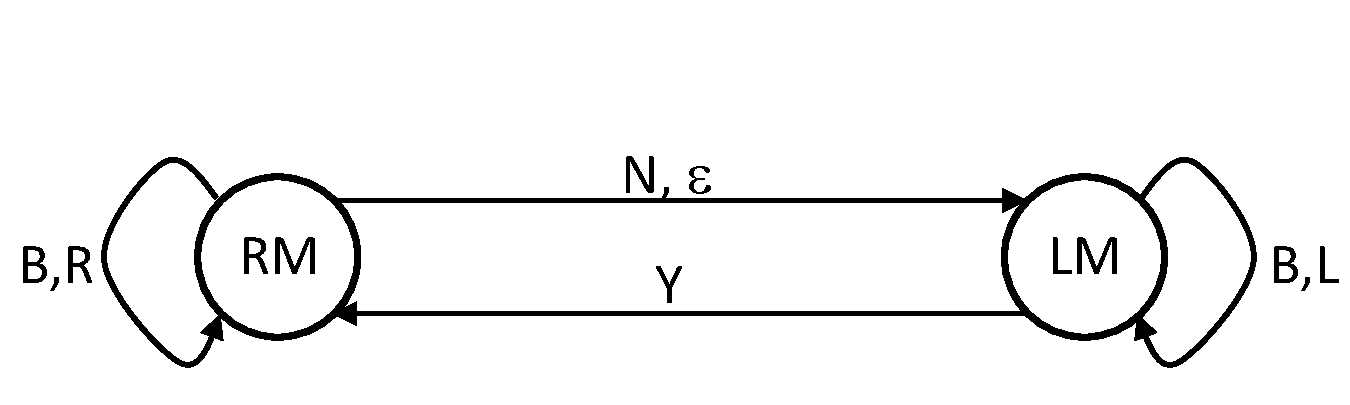
\includegraphics[scale=0.35]{YieldTypeCheckingAutomaton.pdf}
\end{center}
The automaton has two states---$\RM$ and $\LM$.
The edge labels belong to the set $\{B,R,L,N,Y\}$, where $B$, $R$, $L$, and $N$ represent the various kinds 
of atomic actions described earlier, $A$ represents an atomic block, and $Y$ represents a yield.
The judgment $\actions \jy \Prog$ checks that all the code in $\Prog$, except procedures in $\dom(\Refines)$,
can be simulated by traces of this automaton.
This automaton allows traces in which {\em transactions\/} are separated by yields;
each transaction starts with a sequence of right movers (or both movers) and ends with a sequence of left movers (or both movers).
In the middle, it can have at most one non mover.

The essence of the rules in Figure~\ref{fig:yield-sufficiency}
is to capture the effect of a computation as a pair $(x,y)$ where $x,y \in \{\RM,\LM\}$;
the meaning is that to simulate the computation the automaton moves from state $x$ to state $y$.
Rule \textsc{Program} performs checking for all threads and for all procedures not in $\dom(\Refines)$ since these are the 
only procedures that remain in the abstract program.
Rules \textsc{Thread}, \textsc{Stack}, and \textsc{Procedure} are straightforward.
Rule \textsc{While} checks that the body of the loop leaves the state of the automaton unchanged.
Rule \textsc{Ite} checks that the effect both branches is the same.
Rule \textsc{Seq} composes the effect of $\stmt_1$ with the effect of $\stmt_2$.
Rules \textsc{Both}, \textsc{Right}, \textsc{Left}, \textsc{Non}, and \textsc{Ablock} essentially 
examine the available edges in the automaton to validate the statement and calculate its effect.
Rule \textsc{Async} is interesting because it treats an asynchronous call as a left mover.
Rules \textsc{Yield} and \textsc{Call} treat their statements as a yield.
Rule \textsc{Skip} leave the state of the automaton unchanged.

The judgment $\actions \jy \Prog$ is not quite enough to eliminate yields soundly.
Consider the following program with a global variable {\tt x}, two threads, procedure {\tt IncrAndBlock},
and actions {\tt Nop} and {\tt Block}.

{\small
\begin{tabular}{l}
\begin{tabular}{l@{}l@{}l}
\begin{tabular}[t]{l}
{\tt [ x := 0 ];} \\
{\tt [ assert x == 0 ];} \\
\end{tabular} 
&
{\tt ||}
&
\begin{tabular}[t]{l}
{\tt call IncrAndBlock;} \\
\end{tabular} 
\end{tabular} \\
~\\
\begin{tabular}[t]{l}
{\tt procedure IncrAndBlock} \\
{\tt ~~refines Block} \\
{\tt \{} \\
{\tt ~~[ x := x + 1 ];} \\
{\tt ~~while (true)} \\
{\tt ~~~~call Nop;} \\
{\tt \}}
\end{tabular} \\
~\\
\begin{tabular}{l}
{\tt action Nop} \\
{\tt ~~both [ ]}
\end{tabular} \\
~\\
\begin{tabular}{l}
{\tt action Block} \\
{\tt ~~atomic [ assume false ]}
\end{tabular}
\end{tabular}
}

This program violates the assertion in it.
The first thread sets {\tt x} to $0$ in the atomic action indicated {\tt [x := 0]} and yields;
the second thread changes {\tt x} to $1$ and yields;
the first thread fails the assert {\tt x == 0}. 
However, after {\tt call IncrAndBlock} is replaced with the {\tt call Block}, the program does not fail,
even though the code of {\tt IncrAndBlock} satisfies the yield elimination check described earlier and refines the action {\tt Block}.
To address this soundness problem in the presence of left and both movers, we require additionally 
that the abstract program is responsive, that is, it yields infinitely often in any infinite execution.
The abstract program in the example above is not responsive.

\begin{lemma}
Let $\Prog \in \CProgram$ be such that $\vdash \Prog$, $\CommutativitySafe(\Prog)$, and $\jy \Prog$.
If $\Cooperative^*(\Prog)$ and $\CSafe^*(\Prog)$, then $\Safe^*(\Prog)$.
\end{lemma}

\subsection{Refinement}
\label{sec:refinement}

\begin{figure}
\scriptsize{
\medskip
%%%%%%%%%%%%%%%%%%%%
$
\inferrule
{
}
{\actions \vdash \skipstmt \preceq \Havoc(\{\})}
\;(\textsc{Skip})
$
\medskip
%%%%%%%%%%%%%%%%%%%%
$
\inferrule
{
}
{\actions \vdash \yield{e,\lins} \preceq \false}
\;(\textsc{Yield})
$
\medskip
%%%%%%%%%%%%%%%%%%%%
$
\inferrule
{
\actions(A) = (\rho, \alpha, m) 
}
{\actions \vdash \call{A} \preceq \rho \circ \alpha}
\;(\textsc{Atomic})
$
\medskip
%%%%%%%%%%%%%%%%%%%%
$
\inferrule
{
}
{\actions \vdash \call{P} \preceq \false}
\;(\textsc{Call})
$
\medskip
%%%%%%%%%%%%%%%%%%%%
$
\inferrule
{
}
{\actions \vdash \async{P} \preceq \Havoc(\{\})}
\;(\textsc{Async})
$
\medskip
%%%%%%%%%%%%%%%%%%%%
$
\inferrule
{
s \preceq \alpha
}
{\actions \vdash \ablock{e,\lins}{s} \preceq \alpha}
\;(\textsc{Ablock})
$
\medskip
%%%%%%%%%%%%%%%%%%%%
$
\inferrule
{
\actions \vdash \stmt_1 \preceq \alpha_1 \\\\ \actions \vdash \stmt_2 \preceq \alpha_2
}
{\actions \vdash \stmt_1;\stmt_2 \preceq \alpha_1 \circ \alpha_2}
\;(\textsc{Seq})
$
\medskip
%%%%%%%%%%%%%%%%%%%%
$
\inferrule
{
\actions \vdash \stmt_1 \preceq \ga{\locExpr}{\alpha_1} \\ \actions \vdash \stmt_2 \preceq \ga{\neg\locExpr}{\alpha_2}
}
{\actions \vdash \ite{\locExpr}{\stmt_1}{\stmt_2} \preceq \alpha_1 \vee \alpha_2}
\;(\textsc{Ite})
$
\medskip
%%%%%%%%%%%%%%%%%%%%
$
\inferrule
{
\actions \vdash \stmt \preceq \beta \\ \Havoc(\{\}) \subseteq \alpha \\ \beta \circ \alpha \subseteq \alpha 
}
{\actions \vdash \while{e,\alpha}{\locExpr}{\stmt} \preceq e \circ \alpha \circ \neg \locExpr}
\;(\textsc{While})
$
\medskip
%%%%%%%%%%%%%%%%%%%%
$
\inferrule
{
\actions \vdash \stmt \preceq \alpha \\ \alpha \subseteq \alpha'
}
{\actions \vdash \stmt \preceq \alpha'}
\;(\textsc{Weaken})
$
\medskip
}
\caption{Statement summarization}
\label{fig:statement-summarization}
\end{figure}

In this section, we formalize the judgments $\Refines;\SkipProcs \jr \Prog$ and $\InterferenceSafe(\Prog)$.
The rules for the judgment $\Refines;\SkipProcs \jr \Prog$, presented in Figure~\ref{fig:refinement}, check that the body of 
each procedure $P$ in $\dom(\Refines)$ behaves like the atomic action $\Refines(P)$.  
Suppose $P$ is a procedure in $\dom(\Refines)$, $A = \Refines(P)$, and $\actions(A) = (\rho, \alpha, m)$.
Our strategy for $P$ is to check that along all paths in its body, there occurs exactly one atomic block 
$\ablock{e,\lins}{\stmt}$ that is simulated by the transition relation $\alpha$.
All other atomic blocks before or after this unique block are simulated by the transition relation $\Havoc(\Local)$ 
which allows procedure-local variables to be modified arbitrarily but requires that global and thread-local variables are not modified.
The judgment for simulating a code block with a transition relation is $\actions \vdash \stmt \preceq \alpha$; the rules for this judgment 
are presented in Figure~\ref{fig:statement-summarization}.
In general, it may not be possible to prove that the body $\stmt$ of the atomic block is simulated by $\alpha$.
Contextual information such as the predicate $e$ that is expected to hold when the atomic block begins execution or the invariants
of the loop inside the atomic block may also be needed.
Proving such predicates throughout the program is the job of the judgments $\Refines;\SkipProcs \jr \Prog$ and $\InterferenceSafe(\Prog)$.
The rules for the former are presented in Figure~\ref{fig:refinement} and the latter is formalized in text towards the end of this 
subsection.

We first examine the rules for the judgment $\actions \vdash \stmt \preceq \alpha$ in Figure~\ref{fig:statement-summarization}.
The intention of this judgment is to summarize all yield-free and failure-free executions of any statement $\stmt$ by the transition relation $\alpha$.
Since there are no yield and assert statements inside atomic blocks, this judgment is clearly enough for summarizing them;
the extra generality turns out to be useful later in Section~\ref{sec:yield-elimination}.
The rules \textsc{Skip} and \textsc{Async} are similar;
each statement is simulated by the transition relation $\Havoc(\{\})$ which leaves all variables unchanged.
The rules \textsc{Yield} and \textsc{Call} are similar;
each statement is simulated by $\false$ because our goal is to summarize only yield-free executions.
Rule \textsc{Atomic} summarizes the call to an atomic action by the transition relation of the action.
Rule \textsc{Ablock} simply summarizes the code block contained inside the atomic block.
The rule \textsc{Seq} states that if $\stmt_1$ and $\stmt_2$ are simulated by $\alpha_1$ and $\alpha_2$ respectively, 
then $\stmt_1;\stmt_2$ is simulated by the relational composition $\alpha_1 \circ \alpha_2$.
The rule \textsc{Ite} states that if $\stmt_1$ is simulated by $\ga{\locExpr}{\alpha_1}$ and 
$\stmt_2$ is simulated by $\ga{\neg \locExpr}{\alpha_2}$,
then $\ite{\locExpr}{\stmt_1}{\stmt_2}$ is simulated by $\alpha_1 \vee \alpha_2$.
The rule \textsc{While} summarizes the body of the while loop by the transition relation $\beta$ and checks that the 
loop summary $\alpha$ provided by the programmer is inductive.
These checks allow the rule to conclude that the loop is summarized by $e \circ \alpha \circ \neg \locExpr$.
Note that the computed loop summary assumes the loop invariant $e$ since it is checked by the judgments 
discussed later (Figure~\ref{fig:refinement}).

\begin{figure*}
\scriptsize{
\medskip
%%%%%%%%%%%%%%%%%%%%
$
\inferrule
{
}
{\Refines;\SkipProcs;\procs;\actions;P;\{\};b \jr \FH{\phi}{\skipstmt}{\phi};b}
\;(\textsc{Skip})
$
\medskip
%%%%%%%%%%%%%%%%%%%%
$
\inferrule
{
P \not \in \dom(\Refines) \vee P \in \SkipProcs
}
{\Refines;\SkipProcs;\procs;\actions;P;\{\};b \jr \FH{e}{\yield{e,\lins}}{e};b}
\;(\textsc{Yield1})
$
\medskip
%%%%%%%%%%%%%%%%%%%%
$
\inferrule
{
P \in \dom(\Refines) \\ \actions(\Refines(P)) = (\rho, \alpha, m)
}
{\Refines;\SkipProcs;\procs;\actions;P;\{\};b \jr \FH{e}{\yield{e,\lins}}{e \wedge (\rho \vee b)};b}
\;(\textsc{Yield2})
$
\medskip
%%%%%%%%%%%%%%%%%%%%
$
\inferrule
{
\actions(A) = (\rho, \alpha, m) \\\\ 
\mods \subseteq \ThreadLocal \\
\alpha \subseteq \Havoc(\Global \cup \mods \cup \Local) \\\\
P \in \dom(\Refines) \cup \SkipProcs \Rightarrow \phi \subseteq \rho \\ 
\cod((\phi \wedge \rho) \circ \alpha) \subseteq \psi  \\
}
{\Refines;\SkipProcs;\procs;\actions;P;\mods;b \jr \FH{\phi}{\call{A}}{\psi};b}
\;(\textsc{Atomic})
$
\medskip
%%%%%%%%%%%%%%%%%%%%
$
\inferrule
{
P \in \dom(\Refines) \cup \SkipProcs \Rightarrow P' \in \SkipProcs \\
\procs(P') = (\phi, \mods, \psi, \stmt)
}
{\Refines;\SkipProcs;\procs;\actions;P;\mods;b \jr \FH{\phi}{\call{P'}}{\psi};b}
\;(\textsc{Call})
$
\medskip
%%%%%%%%%%%%%%%%%%%%
$
\inferrule
{
P \in \dom(\Refines) \cup \SkipProcs \Rightarrow P' \in \SkipProcs \\
\procs(P') = (\phi, \mods, \psi, \stmt)
}
{\Refines;\SkipProcs;\procs;\actions;P;\{\};b \jr \FH{\phi}{\async{P'}}{\phi};b}
\;(\textsc{Async})
$
\medskip
%%%%%%%%%%%%%%%%%%%%
$
\inferrule
{
P \not \in \dom(\Refines) \cup \SkipProcs \\\\
\Refines;\SkipProcs;\procs;\actions;P;\mods;b \jr \FH{\phi_1 \wedge e}{\stmt}{\phi_2};b
}
{\Refines;\SkipProcs;\procs;\actions;P;\mods;b \jr \FH{\phi_1 \wedge e}{\ablock{e,\lins}{\stmt}}{\phi_2};b}
\;(\textsc{Ablock1})
$
\medskip
%%%%%%%%%%%%%%%%%%%%
$
\inferrule
{
P \in \dom(\Refines) \cup \SkipProcs \\ \actions \vdash \stmt \preceq \ga{e}{\Havoc(\Local)} \\\\
\Refines;\SkipProcs;\procs;\actions;P;\mods;b \jr \FH{\phi_1 \wedge e}{\stmt}{\phi_2};b
}
{\Refines;\SkipProcs;\procs;\actions;P;\mods;b \jr \FH{\phi_1 \wedge e}{\ablock{e,\lins}{\stmt}}{\phi_2};b}
\;(\textsc{Ablock2})
$
\medskip
%%%%%%%%%%%%%%%%%%%%
$
\inferrule
{
P \in \dom(\Refines) \\ \actions(\Refines(P)) = (\rho,\alpha,m) \\\\
\actions \vdash \stmt \preceq \ga{e}{\elim{\Local}.\ \alpha} \\\\
\Refines;\SkipProcs;\procs;\actions;P;\mods;\false \jr \FH{\phi_1 \wedge e}{\stmt}{\phi_2};\false
}
{\Refines;\SkipProcs;\procs;\actions;P;\mods;\false \jr \FH{\phi_1 \wedge e}{\ablock{e,\lins}{\stmt}}{\phi_2};\true}
\;(\textsc{Ablock3})
$
\medskip
%%%%%%%%%%%%%%%%%%%%
$
\inferrule
{
\Refines;\SkipProcs;\procs;\actions;P;\mods_1;b \jr \FH{\locExpr \wedge \phi_1}{s_1}{\phi_2};b' \\\\
\Refines;\SkipProcs;\procs;\actions;P;\mods_2;b \jr \FH{\neg \locExpr \wedge \phi_1}{s_2}{\phi_2};b'
}
{\Refines;\SkipProcs;\procs;\actions;P;\mods_1 \cup \mods_2;b \jr \FH{\phi_1}{\ite{\locExpr}{s_1}{s_2}}{\phi_2};b'}
\;(\textsc{Ite})
$
\medskip
%%%%%%%%%%%%%%%%%%%%
$
\inferrule
{
\Refines;\SkipProcs;\procs;\actions;P;\mods;b \jr \FH{e \wedge \locExpr}{s}{e};b
}
{\Refines;\SkipProcs;\procs;\actions;P;\mods;b \jr \FH{e}{\while{e,\alpha}{\locExpr}{s}}{e \wedge \neg \locExpr};b}
\;(\textsc{While})
$
\medskip
%%%%%%%%%%%%%%%%%%%%
$
\inferrule
{
\phi \subseteq \phi' \\ \psi' \subseteq \psi \\\\
\Refines;\SkipProcs;\procs;\actions;P;\mods;b \jr \FH{\phi'}{\StmtStack}{\psi'};b'
}
{\Refines;\SkipProcs;\procs;\actions;P;\mods;b \jr \FH{\phi}{\StmtStack}{\psi};b'}
\;(\textsc{Weaken})
$
\medskip
%%%%%%%%%%%%%%%%%%%%
$
\inferrule
{
\Refines;\SkipProcs;\procs;\actions;P;\mods;b \jr \FH{\phi}{\StmtStack}{\psi};b' \\ \accessVars(\rho) \cap \mods = \{\}
}
{\Refines;\SkipProcs;\procs;\actions;P;\mods;b \jr \FH{\rho \wedge \phi}{\StmtStack}{\rho \wedge \psi};b'}
\;(\textsc{Frame})
$
\medskip
%%%%%%%%%%%%%%%%%%%%
$
\inferrule
{
\Refines;\SkipProcs;\procs;\actions;P;\mods_1;b_1 \jr \FH{\phi_1}{\StmtStack}{\phi_2};b_2 \\\\ 
\Refines;\SkipProcs;\procs;\actions;P;\mods_2;b_2 \jr \FH{\phi_2}{s}{\phi_3};b_3
}
{\Refines;\SkipProcs;\procs;\actions;P;\mods_1 \cup \mods_2;b_1 \jr \FH{\phi_1}{\StmtStack;s}{\phi_3};b_3}
\;(\textsc{Seq})
$
\medskip
%%%%%%%%%%%%%%%%%%%%
$
\inferrule
{
\Refines;\SkipProcs;\procs;\actions;P';\mods;b \jr \FH{\phi'}{\StmtStack}{\psi};b' \\\\
(\accessVars(\phi) \cup \accessVars(\psi)) \cap \Local = \{\} \\\\
\forall \varsG,\varsTL.\ \MakeStore{\varsG}{\varsTL}{\varsL'} \in \phi \Rightarrow \MakeStore{\varsG}{\varsTL}{\varsL'} \in \phi'
}
{
\Refines;\SkipProcs;\procs;\actions;P;\mods;b \jr \FH{\phi}{(P',\varsL',\StmtStack)}{\psi};b'
}
\;(\textsc{Stack})
$
\medskip
%%%%%%%%%%%%%%%%%%%%
$
\inferrule
{
\procs(P) = (\phi, \mods, \psi, \stmt) \\
\mods' \subseteq \mods \\\\
\Refines;\SkipProcs;\procs;\actions;P;\mods';P \not \in \dom(\Refines) \jr \FH{\phi}{\stmt}{\psi};\true
}
{
\Refines;\SkipProcs;\procs;\actions \jr P
}
\;(\textsc{Procedure})
$
\medskip
%%%%%%%%%%%%%%%%%%%%
$
\inferrule
{
T = (\varsTL, (P, \varsL, \StmtStack)) \\
\MakeStore{\varsG}{\varsTL}{\varsL} \in \phi \\
\mods \subseteq \ThreadLocal \\\\
\Refines;\SkipProcs;\procs;\actions;P;\mods;b \jr \FH{\phi}{\StmtStack}{\StateExpr};\true
}
{
\Refines;\SkipProcs;\procs;\actions;\varsG;b \jr T
}
\;(\textsc{Thread})
$
\medskip
%%%%%%%%%%%%%%%%%%%%
$
\inferrule
{
\forall P \in \ProcName.\ \Refines;\SkipProcs;\procs;\actions \jr P \\\\
\forall 1 \le i \le n.\ \Refines;\SkipProcs;\procs;\actions;\varsG;b_i \jr T_i
}
{
\Refines;\SkipProcs;b_1;\ldots;b_n \jr (\procs, \actions, \ProcLins, \varsG, T_1 \ldots T_n)
}
\;(\textsc{Program})
$
\medskip
%%%%%%%%%%%%%%%%%%%%
}
\caption{Refinement}
\label{fig:refinement}
\end{figure*}

Next we examine the rules for the the judgment $\Refines \jr \Prog$ in Figure~\ref{fig:refinement}.
These rules are a generalization of the sequential correctness rules in the Owicki-Gries method.
In addition to checking that annotations such preconditions, postconditions, loop invariants, 
and predicates labeling yield and atomic block statements are correct, it also checks that the bodies
of each procedure $P \in \dom(\Refines)$ is abstracted by the atomic action $\Refines(P)$.
The crux of these rules is the judgment $\Refines;\SkipProcs;\procs;\actions;P;\mods;b \jr \FH{\phi}{\StmtStack}{\psi} : b'$.
In this judgment, $P$ is the procedure being checked.
The set $\mods$ contains thread-local variables that are potentially modified by $\StmtStack$.
The $\mathit{Boolean}$ values $b$ and $b'$ track whether that atomic action to be refined has already occurred;
the refinement checking is performed only if $P \in \dom(\Refines)$.
Suppose $\Refines(P) = A$ and $\actions(A) = (\rho, \alpha, m)$.
If $b$ is $\true$, then an atomic block refining $A$ has already happened before $\StmtStack$ begins execution, 
the judgment checks that all atomic blocks excuted by $\StmtStack$ refine $\Havoc(\Local)$, and $b'$ remains $\true$.
A statement in which all atomic blocks refine $\Havoc(\Local)$ is said to {\em stutter}.
If $b$ is $\false$, then all atomic blocks before $\StmtStack$ begins execution refine $\Havoc(\Local)$,
and $b'$ evaluates to $\true$ if exactly one atomic block in $\StmtStack$ refines $A$.
Finally, on the right side of the judgment we have the standard Floyd-Hoare triple $\FH{\phi}{\StmtStack}{\psi}$ 
indicating that $\StmtStack$ is being verified assuming it executes from a state in $\phi$ and ensuring it ends in a state satisfying $\psi$.
In the discussion below, we will informally refer to the pair $(b,\phi)$ as the precondition and $(b',\psi)$
as the postcondition of $\StmtStack$, respectively.

Starting from the bottom, rule \textsc{Program} checks each thread and each procedure separately.
The rule \textsc{Thread} checks the body of the thread.
The rule \textsc{Procedure} checks the body of the procedure $P$ with
the precondition $(\false,\phi)$ and postcondition $(P \in \dom(\Refines),\psi)$,
where $\phi$ and $\psi$ are the preconditin and postconditions of $P$ respectively.
This check ensures that if $P$ has an atomic action specification, the body refines it appropriately.
The rule \textsc{Stack} eliminates the dependency on local variables from the precondition when a stack frame is popped.
The rules \textsc{Weaken} and \textsc{Frame} are standard.
The rule \textsc{While}, \textsc{Ite}, and \textsc{Seq} extend the analogous Floyd-Hoare rules with refinement checking.
The rule \textsc{While} checks that the body of the loop stutters and concludes that the loop itself stutters.
The rule \textsc{Ite} checks that both branches behave in the same way.
The rule \textsc{Seq} for $\StmtStack;\stmt$ chains the refinement behavior of $\StmtStack$ with that of $\stmt$.

Rules \textsc{Ablock1}, \textsc{Ablock2}, and \textsc{Ablock3} handle an atomic block $\ablock{e,\lins}{s}$.
Rule \textsc{Ablock1} considers the case when $P \not \in \dom(\Refines)$ and performs only the 
standard sequential correctness check.
Rules \textsc{Ablock2} and \textsc{Ablock3} consider the two cases when $P \in \dom(\Refines)$ and handle
the refinement of $\Havoc{Local}$ and the atomic action $\Refines(P)$, respectively.
Both rules use the judgment $\actions \vdash \stmt \preceq \alpha$ from Figure~\ref{fig:statement-summarization}.

Rules \textsc{Call1}, \textsc{Call2}, \textsc{Async1}, and \textsc{Async2} handle procedure calls.
Rule \textsc{Call1} handles an ordinary call when $P \not \in \dom(\Refines)$ and is straightforward.
Rule \textsc{Call2} handles an ordinary call when $P \in \dom(\Refines)$.
This rule requires that the called procedure $P$ must also have an atomic specification;
thus, the set of procedures being introduced during refinement must be closed under the call relation.
Furthermore, the atomic specification of the callee must be of the special form
where the gate is unconstrained and the transition relation does not modify any variable.
These constraints ensure that the execution inside the callee does not interfere with the caller's refinement checking 
which can then be performed locally.
Rules \textsc{Async1} and \textsc{Async2} handle asynchronous calls and are similar to \textsc{Call1} and \textsc{Call2}, respectively.

Rule \textsc{Atomic} handles the call of an atomic action.
It computes the set of thread-local variables possibly modified by the action in $\mods$.
It checks that the gate of the action holds but only when the call occurs inside the body of a procedure 
that is refining an atomic action.
This is adequate for our soundness theorem (Theorem~\ref{thm:correctness}) which concludes the safety of the concrete 
program from the safety of the abstract program.
Thus, if an assertion (gate of an atomic action) remains in the abstract it is safe to leave it unverified.
Finally, this rule verifies the postcondition $\psi$ from the precondition $\phi$ using the semantics of the atomic action.

Rules \textsc{Yield1} and \textsc{Yield2} handle the yield statement.
Rule \textsc{Yield1} considers the case when $P \not \in \dom(\Refines)$ and is straightforward;
only the yield predicate is available in the postcondition of the statement.
Rule \textsc{Yield2} considers the case when $P \in \dom(\Refines)$ and makes available in the postcondition, in 
addition to the yield predicate, the gate of the action being refined.
Again, this is safe because the gate remains as an assertion in the abstract program.

We now discuss the judgment $\InterferenceSafe(\Prog)$,
where $\Prog = (\procs, \actions, \ProcLins, \varsG, \TS)$. 
Let $\Yields(\Prog)$ be the union of the following sets:
\begin{itemize}
\item
$\{(\phi,\lins) \mid \yield{\phi,\lins}~\mathrm{appears~in~\Prog}\}$.
\item
$\{(\phi,\lins) \mid P \in \ProcName \wedge \procs(P) = (\phi, \mods, \psi, \stmt) \wedge \ProcLins(P) = (\lins,\lins')\}$.
\item
$\{(\psi,\lins') \mid P \in \ProcName \wedge \procs(P) = (\phi, \mods, \psi, \stmt) \wedge \ProcLins(P) = (\lins,\lins')\}$.
\end{itemize}
Let $\Ablocks(\Prog)$ be the set of atomic blocks in $\Prog$.
The program $\Prog$ is interference-free, denoted by $\InterferenceSafe(\Prog)$,
if for each predicate ($\phi,\lins_y) \in \Yields(\Prog)$ and 
for each atomic block $\ablock{e,\lins}{\stmt} \in \Ablocks(\Prog)$, there exists $\alpha$ such that 
$\actions \vdash \stmt \preceq \alpha$ and 
\[
\scriptsize{
\begin{array}{l}
\forall \varsG,\varsTL,\varsL,\varsG',\varsTL',\varsL',\varsTL_y,\varsL_y.\\ 
\mathit{let}\ \Lambda =
\begin{array}[t]{ll}
\cup & \Collect(\varsG, \lins \cap \Global) \\
\cup & \Collect(\varsTL, \lins \cap \ThreadLocal) \\
\cup & \Collect(\varsTL_y, \lins_y \cap \ThreadLocal) 
\end{array} \\
\mathit{in}\
\begin{array}{ll}
\wedge & \IsSet(\Lambda) \\
\wedge & \MakeStore{\varsG}{\varsTL}{\varsL} \in e \\
\wedge & (\MakeStore{\varsG}{\varsTL}{\varsL}, \MakeStore{\varsG'}{\varsTL'}{\varsL'}) \in \alpha \\
\wedge & \MakeStore{\varsG}{\varsTL_y}{\varsL_y} \in \phi
\end{array}
\Rightarrow \MakeStore{\varsG'}{\varsTL_y}{\varsL_y} \in \phi.
\end{array}
}
\]

\begin{lemma}
Let $\Prog,\Prog' \in \CProgram$ be such that $\vdash \Prog$ and $\vdash \Prog'$.
Let $\Refines \in \ProcName \pf \ActionName$, $\SkipProcs \in 2^{\ProcName}$, $\AvailableActions \in 2^{\ActionName}$,
and $\bs{b} \in \overrightarrow{\mathit{Boolean}}$ be such that 
$\Refines;\SkipProcs;\AvailableActions;\bs{b} \vdash \Prog \leadsto \Prog'$, $\Refines;\SkipProcs;\bs{b} \jr \Prog$, and
$\InterferenceSafe(\Prog)$.
If $\Safe(\Prog')$, then $\CSafe(\Prog)$.
\end{lemma}

\begin{lemma}
Let $\Prog_1,\Prog_2,\Prog'_1 \in \CProgram$ be such that $\vdash \Prog_1$, $\vdash \Prog'_1$,
and $\Prog_1 \ctrans \Prog_2$.
Let $\Refines \in \ProcName \pf \ActionName$, $\SkipProcs \in 2^{\ProcName}$, $\AvailableActions \in 2^{\ActionName}$,
and $\bs{b_1} \in \overrightarrow{\mathit{Boolean}}$ be such that 
$\Refines;\SkipProcs;\AvailableActions;\bs{b_1} \vdash \Prog_1 \leadsto \Prog'_1$, $\Refines;\SkipProcs;\bs{b} \jr \Prog_1$, and
$\InterferenceSafe(\Prog_1)$.
If $\Safe(\Prog')$, then there exists $\Prog'_2 \in \Program$ and $\bs{b_2} \in \overrightarrow{\mathit{Boolean}}$ such that 
$\Prog_2 \trans^* \Prog'_2$, $\Refines;\SkipProcs;\AvailableActions;\bs{b_2} \vdash \Prog_2 \leadsto \Prog'_2$, 
$\Refines;\SkipProcs;\bs{b_2} \jr \Prog_2$, and $\InterferenceSafe(\Prog_2)$.
\end{lemma}


{\bf Proving cooperation.}
Given a program $\Prog \in \CProgram$, proving $\Cooperative^*(\Prog)$ 
is similar to proving termination of sequential program.
The basic idea is to provide a loop with a measure function $f$ that decreases for each yield-free and failure-free 
execution of the body of the loop.
Thus, we can prove responsivenes by modifying only \textsc{While} rule in Figure~\ref{fig:refinement}
as follows:
\[
\scriptsize{
\inferrule
{
\Refines;\SkipProcs;\procs;\actions;P;\mods;b \jr \FH{e \wedge \locExpr}{s}{e};b \\\\
\rho = \{ \sigma \mid \sigma(f) \geq 0 \} \\
e \wedge \locExpr \subseteq \rho \\\\
\alpha = \{(\sigma,\sigma') \mid \sigma(f) > \sigma'(f)\} \\
\actions \vdash \stmt \preceq \ga{(e \wedge \locExpr)}{\alpha}
}
{\Refines;\SkipProcs;\procs;\actions;P;\mods;b \jr \FH{e}{\while{e,\alpha,f}{\locExpr}{\stmt}}{e \wedge \neg \locExpr};b}
}
\]
